\documentclass[12pt,oneside,letterpaper,spanish]{article}
\usepackage[T1]{fontenc}
\usepackage{csquotes}
\usepackage[utf8]{inputenc}
\usepackage[margin=2.25cm,headheight=26pt,includeheadfoot]{geometry}
\usepackage[spanish]{babel}
\usepackage{listings}
\usepackage{color}
\usepackage{titlesec}
\usepackage{titling}
\usepackage[framed, numbered]{matlab-prettifier}
\usepackage{changepage}
\usepackage{amsmath}
\usepackage{hyperref}
\usepackage{enumitem}
\usepackage{graphicx}
\usepackage{fancyhdr}
\usepackage{lastpage}
\usepackage{caption}
\usepackage{tocloft}
\usepackage{setspace}
\usepackage{multirow}
\usepackage{titling}
\usepackage{float}
\usepackage{comment}
\usepackage{booktabs}
\usepackage{indentfirst}
\usepackage{lscape}
\usepackage{booktabs,caption}
\usepackage[flushleft]{threeparttable}
\usepackage[english]{nomencl}
\usepackage{xcolor}
\usepackage{lipsum}
\usepackage{array}
\usepackage{natbib}
\usepackage{tikz}

% --- set footer and header ---
\pagestyle{fancy}
\fancyhf{}

\setlength{\parindent}{2em}
\title{Bitácora 1} % to reference as \title, dont use \maketitle
\makeatletter\let\Title\@title\makeatother



\lstset{language=Matlab,
style=Matlab-editor,
basicstyle=\normalsize\mlttfamily,
numbers=left,
numberstyle={\scriptsize\color{black}},	% size of the numbers
numbersep=0.5cm											
}

\newlist{steps}{enumerate}{1}
\setlist[steps, 1]{leftmargin=1.5cm,label = Step \arabic*:}
\renewcommand{\headrulewidth}{1pt}
\renewcommand{\footrulewidth}{1pt}
\renewcommand{\rmdefault}{ptm}

%\lhead{\Title}
\rhead{\nouppercase{\rightmark}}
\lhead{\Title}
\setlength\headheight{16pt}
\setlength{\footskip}{50pt}
\lhead{\Title} %rightH title
\cfoot{\thepage}

% --- End of page settings ---


\begin{document}
\pagenumbering{roman} 
\begin{titlepage}
\begin{center}
\vspace{2cm}

\includegraphics[width=0.2\textwidth]{root/Logo_ucr.png}~\\[1cm]

{\huge Universidad de Costa Rica} \\
{\large 
Escuela de Matemáticas \\
Estadística Actuarial I \\
CA-0303\\
}

\vspace{.5cm}


\hrule
\vspace{.5cm}
{ \Huge \bfseries Proyecto - Bitácora II} 
\vspace{.5cm}
\hrule
\vspace{1cm}

{\Large \textbf{Relación entre los indicadores de progreso socioeconómico y el índice de felicidad de los países}}
\vspace{1cm}

\textsc{\textbf{Profesor}}\\
\vspace{2px}

Maikol Solís Chacón PhD \\

\vspace{.5cm}
\textsc{\textbf{Estudiantes}}\\
\vspace{2px}


Luis Fernando Amey Apuy - C20470\\
\vspace{5px}
Anthony Jiménez Navarro - C24067\\
\vspace{5px}
Javier Hernández Navarro - C13674\\
\vspace{5px}
Erick Venegas Espinoza - C09319\\

\vspace{1cm}

I - 2024 \\


\end{center}
\end{titlepage}

\newpage
\doublespacing
%\addcontentsline{toc}{section}{Table of Contents}
\renewcommand{\baselinestretch}{1}\normalsize
\tableofcontents
\renewcommand{\baselinestretch}{1}\normalsize
%\singlespacing
\thispagestyle{fancy} % force page style

\newpage
\pagenumbering{arabic} 
\fancyfoot[C]{Página \thepage\ de \pageref{EndOfText}}


%
% --- Acá inicia el documento ---
%

\section{Parte de planificación} \label{ch1}

\subsection{Pregunta de investigación}

\subsubsection{Definición de la idea}
% Factores relacionados con el progreso en los distintos países del mundo.

La idea central es examinar si existe una relación entre el progreso socioeconómico de un país (representado por variables como acceso a la electricidad, PIB per cápita, tasa de alfabetización de adultos, entre otros) y el índice de felicidad de sus habitantes. 

Además, se buscará identificar la distribución de la variable aleatoria del índice de felicidad para así comprender mejor su comportamiento y potencialmente obtener información sobre factores predictivos o determinantes de la misma en contextos socioeconómicos.  

\begin{itemize}
    \item \textbf{Están interesados en el tema:} El interés en este tema radica en la comprensión de cómo el progreso socioeconómico de un país se relaciona con el bienestar y la felicidad de sus ciudadanos. Al entender mejor las conexiones entre estos aspectos, podemos identificar áreas de mejora, diseñar estrategias de desarrollo más inclusivas y equitativas, y promover un crecimiento económico que beneficie verdaderamente a toda la sociedad.

    \item \textbf{Es relevante bajo el contexto del curso:} Este tema es relevante ya que proporciona una oportunidad de aplicar los conceptos y técnicas aprendido en clase en un contexto real y significativo. La exploración de la relación entre el progreso socioeconómico y la felicidad de una población implica analizar múltiples variables y entender cómo se distribuye la variable aleatoria de la felicidad.

    \item \textbf{Ya hicieron una investigación rápida del tema:} Sí, y afortunadamente es un tema que ofrece una amplia gama de resultados, desde artículos científicos publicados por universidades, comparaciones entre países por región, estudios de gran relevancia, entre otros.

    \item \textbf{Es una idea específica, pero no demasiado en caso de querer abordar otros métodos o puntos de vista:} El tema en sí ofrece un amplio panorama para investigar, ya que a partir de los indicadores de bienestar de cada país, se pueden llevar a cabo múltiples enfoques para diversas investigaciones. En este caso, al centrarnos en buscar una relación entre el progreso económico y el índice de felicidad, y también determinar la distribución de la misma, estaríamos delimitando el tema, pero siempre dejando abierta la opción de agregar o profundizar más en todo el panorama que ofrece. 
\end{itemize}

\newpage
\subsubsection{Conceptualización de la idea}

\begin{itemize}
    \item \textbf{Relación:} Establecer una conexión entre persona, cosa, ideas o hechos.
    
    \item \textbf{Progreso:} Avance, adelanto o perfeccionamiento.

    \item \textbf{Socioeconómico:} Perteneciente o relativo a los factores sociales y económicos.
    
    \item \textbf{País:} Territorio, con características geográficas y culturales propias, que puede constituir una entidad política dentro de un Estado

    \item \textbf{Índice de felicidad:} El índice global de felicidad es una publicación anual de las Naciones Unidas que mide la felicidad en 187 países, basándose en encuestas a ciudadanos donde estos evalúan su propia vida y sus respuestas se relacionan con distintos factores de calidad de vida.

    \item \textbf{Habitantes:} Cada una de las personas que constituyen la población de un barrio, ciudad, provincia o nación.

    \item \textbf{Distribución:} Una distribución de probabilidad es aquella que permite establecer toda la gama de resultados probables de ocurrir en un experimento determinado.

    \item \textbf{Variable aleatoria:} Valor numérico que corresponde a un resultado de un experimento aleatorio. 

    \item \textbf{Comportamiento:} Se trata de la forma de proceder de las personas u organismos frente a los estímulos y en relación con el entorno.

    \item \textbf{Información:} conjunto organizado de datos relevantes para uno o más sujetos que extraen de él un conocimiento.

    \item \textbf{Factores:}  elemento que juega un rol determinante en un resultado.

    \item \textbf{Predictivos:} aquello que predice o que resulta útil para tal fin hace mención a anticiparse a algo que va a suceder
    
\end{itemize}

\newpage
\subsubsection{Identificación de tensiones}
El acceso a las necesidades básicas esenciales, como lo son el suministro de agua potable, la electricidad, aire libre de contaminación e internet, sigue siendo un privilegio que no todos en el mundo pueden disfrutar. Esta falta de acceso a servicios indispensables para el desarrollo integral afecta a diversas poblaciones a lo largo de las distintas naciones.  

A su vez en muchas naciones, la capacidad de proporcionar empleo a todos los residentes es una tarea la cual no se cumple en su totalidad, lo que resulta en distintos niveles de desempleo o subempleo a lo largo del globo. Esta situación crea tensiones sociales y económicas, perpetuando ciclos de pobreza y desigualdad en las distintas sociedades.  

Además, la alfabetización no es universal incluso en los países más desarrollados, lo cual genera disparidades educativas esto en combinación con la falta de acceso equitativo a oportunidades de aprendizaje genera brechas que separan a los distintos estratos que conforman las sociedades. Esto provoca grupos altamente marginalizados los cuales se encuentran limitados en sus oportunidades para integrarse a las sociedades modernas.  

La corrupción es una afectación presente en empresas internacionales y gobiernos que genera dificultades para un desarrollo integral pleno. La desviación de recursos públicos para el mejoramiento de las condiciones de grupos marginados así como los abusos de autoridad, la falta de responsabilidad y transparencia provoca desconfianza por parte de las poblaciones hacia los gobiernos de turno, generando a su vez un deterioro en la cohesión social.  

\subsubsection{Reformulación de la idea en forma de pregunta}
\begin{itemize}
    \item ¿Existe una relación positiva entre el PIB per cápita y el índice de felicidad de las personas?
    \item ¿De qué manera resulta importante el progreso socioeconómico para un país?
    \item ¿Cómo se relacionan las variables socioeconómicas con el índice de felicidad?
    \item ¿Resulta relevante la distribución del índice de felicidad para conocer otros factores?
\end{itemize}

\newpage
\subsubsection{Argumentación de las preguntas}

\textbf{Pregunta 1:} ¿Existe una relación positiva entre el PIB per cápita y el índice de felicidad de las personas?
\begin{itemize}
    \item Contraargumentos:
    \begin{itemize}
        \item \textbf{Lógica}: La relación que puede existir entre el PIB per cápita y el índice de felicidad de las personas puede ser un proceso más complejo. La distribución desigual que puede experimentar este podría significar que no todos los habitantes de un territorio gocen de un aumento en el índice de felicidad.
        \item \textbf{Ética}: El utilizar el crecimiento económico como medida del progreso de una sociedad y su relación con la felicidad de sus habitantes pueden ser contraproducente, ya que el avance económico tiene relación con la explotación de recursos naturales y una falta de consideración con respecto al bienestar social a expensas de un mayor beneficio económico.
        \item \textbf{Emocional}: Un enfoque central en el desarrollo economico podría resonar de forma negativa para poblaciones de estratos sociales marginalizados, asi como para los individuos que se encuentran en situaciones laborales inadecuadas o en un estado de explotacion laboral.
    \end{itemize}
    \item Argumentos:
    \begin{itemize}
        \item \textbf{Lógica}: El PIB per cápita representa un componente importante para medir el desarrollo de territorios. De igual forma, países mas desarrollados tienden a presentar un PIB per cápita mayor, además de servicios médicos de calidad superior en comparación a países subdesarrollados, lo cual se relaciona de forma positiva con el índice de felicidad a lo largo del planeta.
        \item \textbf{Ética}: Con gobiernos transparentes, un aumento del PIB per cápita, se vería reflejado un aumento equitativo generalizado del bienestar social, lo que a su vez ha demostrado presentar una relación positiva con respecto a la felicidad reportada de los individuos.
        \item \textbf{Emocional}: Aunque la relación existente entre el aumento del bienestar económico y la felicidad se observa como un proceso complejo y polifacético, el aumento del PIB per cápita tiene un efecto directo en la seguridad económica de los habitantes así como un sentimiento de estabilidad.
    \end{itemize}
    \item Conclusión: La relación existente entre el PIB per cápita es un proceso complejo y polifacético. Aunque este puede tener cierta influencia sobre la felicidad, es necesario llevar a cabo un análisis más complejo que tome en cuenta una multiplicidad de variables distintas, tanto situaciones éticas, emocionales como sociales y económicas.
\end{itemize}

\newpage
\textbf{Pregunta 2:} ¿De qué manera resulta importante el progreso socioeconómico para un país?
\begin{itemize}
    \item Contraargumentos: 
    \begin{itemize}
        \item \textbf{Lógica}: La relevancia del progreso socioeconómico puede no resultar de gran importancia para un país, dados muchos casos y contextos. La estabilidad política de un país o ambiental son cruciales en las últimas décadas, para prevenir guerras o desastres ecológicos. En conjunto a eso, la importancia puede ser variada, dependiendo de muchos factores y no solo apuntando a uno central.  
        \item \textbf{Ética}: El progreso socioeconómico puede resultar subjetivo, inclusive entre las variables tomadas en cuenta en el estudio, por lo que se debe continuar con precaución para no presentar una conclusión específica, puesto que se puede excluir algunos grupos selectos.
        \item \textbf{Emocional}: La implementación de la metodología en cuestión puede ser inadecuada e imprecisa en general, donde el progreso socioeconómico puede no reflejar las problemáticas reales del país.
    \end{itemize}
    \item Argumentos:
    \begin{itemize}
        \item \textbf{Lógica}: Es crucial el progreso tanto social como económico en un país, puesto que al mismo tiempo que se crece en recursos económicos y hay más poder adquisitivo y por lo tanto comodidad, la sociedad crece en volumen y entrelaza conexiones entre ellos, haciendo más fácil la comunicación y divulgación de ideas productivas en el sistema. 
        \item \textbf{Ética}: Se cuenta con una gran variedad de factores para poder argumentar sobre un progreso socioeconómico, en general, se puede basar no solo al progreso como univariable pero desde diferentes puntos de vista, como lo puede ser la percepción de corrupción, apoyo social, recursos básicos, entre otros.
        \item \textbf{Emocional}: Lograr observar y detallar sobre los aspectos importantes del desarrollo socioeconómico de un país puede hacer enfocar sobre esos puntos relevantes, y así enfatizar el cuidado de ellos.
    \end{itemize}
    \item Conclusión: Concretar las diferentes importancias del progreso socioeconómico de un país puede contar con muchos enfoques y puntos de vista, así que se debe intentar de dar un análisis general de los datos para poder establecer una conclusión que abarque la realidad de muchos países, inclusive de territorios más pequeños.
\end{itemize}

\newpage
\textbf{Pregunta 3:} ¿Cómo se relacionan las variables socioeconómicas con el índice de felicidad?
\begin{itemize}
    \item Contraargumentos:
    \begin{itemize}
        \item \textbf{Lógica}: Hay evidencia que es ambigua por lo que no podemos determinar a ciencia cierta de que esta vez se va a realizar de manera precisa. Al tratarse de una variable que no es fácil de cuantificar hay que tomar muchos supuestos, sobre qué hace feliz a las personas y pensar que todas las personas racionales, es decir, reducimos en un gran número la población de estudio y ya no sería algo representativo de la población.
        \item \textbf{Ética}: Como se mencionó en el argumento anterior, la variable "felicidad" es subjetiva de cada persona, trata de modelar ésta como una ecuación matemática dejaría por fuera más factores por los cuales las personas son felices. 
        \item \textbf{Emocional}: No podemos encasillar a todas las personas como que solo los beneficios económicos las hacen estar bien, pues éstas mismas pueden tener mucho dinero, que haya poca inflación o que no haya corrupción y aún así no ser felices, esto va más allá y hasta posee matices filosóficos, pues deberíamos empezar por definir "¿Qué es la felicidad?", y si le damos un determinado valor, quién determina que nos hace feliz en la misma magnitud.
    \end{itemize}
    \item Argumentos:
    \begin{itemize}
        \item \textbf{Lógica}: Desde el punto de vista político, tener que en realidad los factores socioeconómicas afectan a la felicidad, puede servir para enfocar esfuerzos a tratar de mejorar la felicidad de las personas y por ende tratar de potenciar su desarrollo. 
        \item \textbf{Ética}: Aunque la relación existente entre los factores socioeconómicos y el índice de felicidad pueda verse como un proceso complejo y  polifacético a lo largo del globo se han desarrollado estudios que relacionan de forma positiva un mayor índice de felicidad con respecto a poblaciones que gozan de mejores oportunidades educativas y salariales así como formar parte de un estrato social superior. 
        \item \textbf{Emocional}: Desde el punto de vista de las personas, tiene gran utilidad saber esto, pues si bien, aunque cada persona tiene una diferente interpretación de felicidad, tener evidencia de que por el lado socioeconómico se puede potenciar ésta, entonces se podría tener una idea de por dónde buscar mejorar.
    \end{itemize}
    \item Conclusión: Aunque medir la felicidad como una ecuación matemática represente problemas, hay un agregado de factores que se pueden tomar en común para tratar de modelar ésta y tratar de enfocar los esfuerzos a mejorar la feclidad de las personas y por ende su calidad de vida.
\end{itemize}

\newpage
\textbf{Pregunta 4:} ¿Resulta relevante la distribución del índice de felicidad para conocer otros factores?
\begin{itemize}
    \item Contraargumentos:
    \begin{itemize}
        \item \textbf{Lógica}: La distribución del índice de felicidad puede no ser relevante para conocer otros factores si no existe una relación clara entre el índice de felicidad y los factores socioeconómicos que se están analizando. Es posible que la felicidad sea influenciada por una serie de variables subjetivas y culturales que no estén directamente relacionadas con el acceso a la electricidad, el PIB per cápita o la tasa de alfabetización de adultos. 
        \item \textbf{Ética}: Es importante considerar que la distribución del índice de felicidad puede ser influenciada por sesgos culturales, sociales y personales, lo que podría distorsionar su interpretación. Además, la medición de la felicidad es intrínsecamente subjetiva y puede estar influenciada por factores temporales y contextuales.
        \item \textbf{Emocional}: Puede resultar desalentador basar la compresión de factores socioeconómicos importantes únicamente en la distribución del índice de felicidad. Esto se debe a que la felicidad es un concepto multifacético y subjetivo que puede ser difícil de cuantificar y comparar entre diferentes culturas y contextos.
    \end{itemize}
    \item Argumentos:
    \begin{itemize}
        \item \textbf{Lógica}: Numerosos estudios han demostrado consistentemente una fuerte correlación entre el bienestar subjetivo de los individuos y diversos aspectos socioeconómicos. Por ejemplo, investigaciones como el World Happiness Report han encontrado que países con mayores ingresos per cápita, mejores sistemas de salud y educación, así como menores niveles de desigualdad tienden a reportar niveles más altos de felicidad en sus poblaciones.
        \item \textbf{Ética}: Considerar la distribución del índice de felicidad es relevante y necesario para comprender otros factores socioeconómicos, siempre y cuando se utilicen métodos de investigación rigurosos y se asegure la integridad de los datos. 
        \item \textbf{Emocional}: Reconocer la importancia de la distribución del índice de felicidad puede generar esperanza y motivación para implementar políticas y programas que mejoren el bienestar de la población. Al centrarse en mejorar los indicadores de felicidad, los gobiernos y las organizaciones pueden abordar aspectos clave como la equidad en la distribución de recursos, el acceso a servicios básicos y la calidad de vida de los ciudadanos. 
    \end{itemize}
    \item Conclusión: La distribución del índice de felicidad es crucial para comprender otros aspectos socioeconómicos, respaldada por evidencia que muestra una fuerte correlación entre el bienestar subjetivo y la calidad de vida. Optar por este enfoque se justifica por su potencial para informar políticas que mejoren la equidad y el bienestar social.
\end{itemize}

\newpage
\subsubsection{Argumentación a través de datos}

\begin{itemize}
    \item \textbf{Fuente de información}: Se cuenta con la base de datos \textit{World Development Data}, la cual es un compilado de métricas obtenidas de \textit{The World Bank} (2018), \textit{World Happiness Report} (2018) y \textit{Transparency International} (2018). \\
    En adición con esta base de datos, se encontró una base de datos original de \textit{World Happiness Report}, en donde aparecen más variables de carácter social, la mayoría numéricas, inclusive trayendo una percepción de felicidad, la cual se usará como índice de felicidad principalmente. Esta base de datos se mezclará bien con la principal, aunque por el momento se describirá solo la principal. 
    \item \textbf{Contexto temporal y espacial de los datos}: Datos recopilados desde el 2014 hasta el 2018, abarcando un total de 186 países.
    \item \textbf{Facilidad de obtener la información}: Alta, la información se encuentra tanto en los repositorios públicos de \textit{The World Bank}, \textit{World Happiness Report} y \textit{Transparency International} así como en \textit{Kaggle}.
    \item \textbf{Población de estudio}: Países que conforman el mundo.
    \item \textbf{Muestra observada}: Participantes de los censos nacionales tomados en cuenta por \textit{The World Bank}, \textit{World Happiness Report} y \textit{Transparency International}.
    \item \textbf{Unidad estadística o individuos}: Países.
    \item \textbf{Descripción de las variables de la tabla}:
    \begin{itemize}
        \item \textbf{country}: País de estudio. Son strings en la tabla de datos.
        \item \textbf{electricity\_access}: Porcentaje de la población que tiene acceso a la electricidad. Es una variable tipo numérica.
        \item \textbf{gdp}: Producto interno bruto expresado en dólares. Es una variable tipo numérica.
        \item \textbf{gdp\_capita}: Producto interno bruto per cápita expresado en dólares. Es una variable tipo numérica.
        \item \textbf{labor\_rate}: Porcentaje de la población que forma parte de la fuerza laboral (mayores de 15 años). Es una variable tipo numérica.
        \item \textbf{labor\_force}: Fuerza laboral total. Es una variable tipo numérica.
        \item \textbf{land\_area}: Tamaño del territorio nacional expresado en kilómetros cuadrados. Es una variable tipo numérica.
        \item \textbf{life\_expectancy}: Esperanza de vida expresado en años. Es una variable tipo numérica.
        \item \textbf{adult\_literacy}: Porcentaje de alfabetización adulta(mayores de 15 años). Es una variable tipo numérica.
        \item \textbf{water\_access}: Porcentaje de la población que tiene acceso al agua potable. Es una variable tipo numérica.
        \item \textbf{air\_pollution}: Porcentaje de la población expuesta a un nivel de aire contaminado establecido por la Organización Mundial de la Salud. Es una variable tipo numérica.
        \item \textbf{population\_density}: Densidad de la población, expresado en personas por kilómetro cuadrado. Es una variable tipo numérica.
        \item \textbf{population}: Población total. Es una variable tipo numérica.
        \item \textbf{alcohol\_consumption}: Consumo de alcohol per cápita. Es una variable tipo numérica.
        \item \textbf{unemployment\_rate}: Tasa de desempleo. Es una variable tipo numérica.
        \item \textbf{social\_support}: Índice del apoyo social reportado por World Happiness Report. Es una variable tipo numérica.
        \item \textbf{freedom}: Índice de libertad para tomar decisiones de vida reportada por World Happiness Report. Es una variable tipo numérica.
        \item \textbf{generosity}: Índice de generosidad reportada por World Happiness Report. Es una variable tipo numérica.
        \item \textbf{income\_class}: Clase social como variable categorica
        \item \textbf{cpi}: Índice de percepción de corrupción expresado del 0 al 100. Es una variable tipo numérica.
    \end{itemize}
\end{itemize}

\newpage
\subsection{Revisión bibliográfica}
\subsubsection{Construcción de fichas de literatura}

\begin{table}[htbp]
    \caption{Ficha de Literatura 1}
    \begin{center}
        \begin{tabular}{  m{3cm} | m{12cm}  }
        \hline\textbf{ Encabezado} & \textbf{Contenido }\\ \hline
        Título: & Movilidad social, preferencias redistributivas y felicidad en Colombia. \\ \hline
        Autor(es): & Juliana Londoño Vélez \\ \hline
        Año: & 2011 \\ \hline
        Nombre del tema: & La movilidad social como uno de los determinantes de la felicidad. \\ \hline
        Cronológica: &  1969-2011 \\ \hline
        Metodológica: & Recolección, comparación, correlación y análisis de datos. \\ \hline
        Temática: & Estudios económicos y psicológicos \\  \hline
        Teórica: & Economía social \\ \hline
        Resumen en una oración: & Quiénes son más felices dadas las determinantes de ingreso, movilidad social y justicia social. \\ \hline
        Argumento central: &  Observar cuál es el estrato que posee mayor felicidad con respecto a la movilidad, ingreso y justicia social \\ \hline
        Problemas con el argumento o el tema: & Existe un pesimismo en la cultura colombiana que provoca que los datos estén sesgado, además de que dicho por el propio estudio, hay un altruismo generacional que afecta en la función de utilidad, es decir, que puede sobrestimar la felicidad de los colombianos. \\ \hline
        Resumen en un párrafo: & El estudio busca relacionar los determinantes de ingreso, movilidad social e injusticia social con el nivel de felicidad de sus habitantes, tratando de hacer un empate entre los resultados empíricos del estudio con las observaciones teóricas que han tenido otros contemporáneos. El estudio logra el objetivo de validar algunas observaciones teóricas, pero contradiciendo otras, además de encontrar que el nivel de ingreso si motiva a la felicidad, pero que no influye en las políticas de redistribución de la riqueza. \\ \hline
        \end{tabular}
    \end{center}
\end{table}

\begin{table}[htbp]
    \caption{Ficha de Literatura 2}
    \begin{center}
        \begin{tabular}{  m{3cm} | m{12cm}  }
        \hline\textbf{ Encabezado} & \textbf{Contenido }\\ \hline
        Título: & ¿Suponen las directrices politicoeconómicas del Reino de Bután, que orientan su objetivo hacia la felicidad de los ciudadanos, un modelo a seguir para los Gobiernos a nivel internacional? \\ \hline
        Autor(es): &  Ignacio Aguilar, Oriol-Jordi Andrés, Guillem Foucault, Ferran Montserrat y Andreu Tixis\\ \hline
        Año: & 2014-2015 \\ \hline
        Nombre del tema: & La economía de Bután, el FIB y el PIB, destacándose entre muchas economías: parte del cuerpo analítico del documento \\ \hline
        Cronológica: & 1980 - 2013 \\ \hline
        Metodológica: & Análisis de datos y correlación sobre índices \\ \hline
        Temática: & Estudios económicos y psicológicos \\ \hline
        Teórica: & Economía social \\ \hline
        Resumen en una oración: & Los países presentan una correlación negativa de felicidad y crecimiento económico, exceptuando el caso de Bután \\ \hline
        Argumento central: & Impacto económico a la felicidad, considerando los factores adversos \\ \hline
        Problemas con el argumento o el tema: & Los índices de felicidad son relativamente nuevos, que en cuestión de análisis, no hay un amplio set de datos para indicar una correlación más contundente. Considerando también que la felicidad es de carácter subjetivo.  \\ \hline
            Resumen en un párrafo: & Bután tuvo un crecimiento económico bastante significativo entre los años 1980-2013, espacio en que se realiza el análisis. Esta economía se destaca entre sus vecinos, inclusive teniendo el segundo crecimiento más alto en todo el mundo por un momento. Además, la felicidad interna bruta (FIB) de Bután también destaca. La investigación intenta hacer una correlación entre las variables para intentar postular a la economía dada como ejemplar, y dado esto logra intuir que, por ejemplo, una gran riqueza no implica una felicidad más grande. El estudio compara con Nepal, Bangladesh, en métodos cercanos porque son economías similares, y también con economías grandes, donde se logra ver que Bután se comporta en correlación de manera distinta al mundo, donde entre más crecimiento económico se logre, más alto es el índice de felicidad.   \\ \hline
        \end{tabular}
    \end{center}
\end{table}

\newpage


\newpage
\begin{table}[H]
    \caption{Ficha de Literatura 3}
    \begin{center}
        \begin{tabular}{  m{3cm} | m{12cm}  }
        \hline\textbf{ Encabezado} & \textbf{Contenido }\\ \hline
        Título: & Salud y Felicidad en Uruguay \\ \hline
        Autor(es): & Mariana Gerstenblüth, Todd Jewell y Máximo Rossi  \\ \hline
        Año: & 2010 \\ \hline
        Nombre del tema: & Estudio de la relación existente entre la felicidad del individuo y el estado de salud auto reportado en Uruguay. \\ \hline
        Cronológica: & 2008-2010 \\ \hline
        Metodológica: & Análisis de datos y correlación entre variables \\ \hline
        Temática: & Estudios económicos y psicológicos \\ \hline
        Teórica: & Economía Social \\ \hline
        Resumen en una oración: & Correlación positiva entre distintas variables y felicidad en Uruguay durante el 2008. \\ \hline
        Argumento central: & Relación positiva existente entre el estado de salud y la felicidad auto reportada, además del impacto de diversas variables en la variable de felicidad autopercibida \\ \hline
        Problemas con el argumento o el tema: & La dificultad mas presente a lo largo de la investigación es la endogeneidad, la cual se observa como una correlación entre un parametro y un termino de error, la cual puede resultar en estimaciones sesgadas. Ademas, variables como la educación, ingreso, estado civil tambien presentan influencie en el calculo de la felicidad, lo que puede generar complicaciones a la hora de encontrar una relacion con esta  \\ \hline
        Resumen en un párrafo: & El estudio analiza la relación que existe entre el estado de salud y felicidad auto percibida, en el territorio de Uruguay a lo largo del año 2008. Se asocia el hecho de gozar de un buen estado de salud con un nivel mas alto de felicidad, siendo este a su vez, uno de los mayores determinantes de la felicidad. Se realiza un estudio además de diversas variables como lo son: desempleo, completación de la educación terciaria, religiosidad, asi como factores socioeconomicos con la felicidad. Se estudia la influencia que puede representar la endogeneidad para encontrar una relación con respecto a la felicidad. Finalmente se concluye con la importancia que representa el estado de salud con respecto a la felicidad en Uruguay.
        \\ \hline
        \end{tabular}
    \end{center}
\end{table}
\newpage
\begin{table}[H]
    \caption{Ficha de Literatura 4}
    \begin{center}
        \begin{tabular}{  m{3cm} | m{12cm}  }
        \hline\textbf{ Encabezado} & \textbf{Contenido }\\ \hline
        Título: &  Crecimiento económico, progreso social y felicidad\\ \hline
        Autor(es): & Luisa Montuschi  \\ \hline
        Año: &  2017\\ \hline
        Nombre del tema: &  La relevancia de incluir un índice de felicidad para medir el progreso socioeconómico de los países. \\ \hline
        Cronológica: &  2012 - 2017\\ \hline
        Metodológica: &  Análisis de datos y una correlación entre los factores determinantes de la felicidad \\ \hline
        Temática: & Estudios ecónomicos y psicológicos \\ \hline
        Teórica:  & Economía \\ \hline
        Resumen en una oración: &  Se ha cuestionado la eficacia del PIB como indicador de progreso social en el siglo XXI, surgiendo la necesidad de desarrollar nuevos indicadores como el Social Progress Index y el Gross National Happiness Index.\\ \hline
        Argumento central: &  Darle un peso significativo al índice de felicidad de los países, y no solo tomar el PIB como referencia de crecimiento socioeconómico.\\ \hline
        Problemas con el argumento o el tema: &  La dificultad para llegar a un consenso global sobre qué aspectos deben incluirse en estos nuevos indicadores de progreso social y cómo medirlos de manera precisa y equitativa. Además, la dicotomía existente en el pensamiento de que el dinero garantiza felicidad.\\ \hline
        Resumen en un párrafo: & En el siglo XXI, se ha cuestionado la capacidad del Producto Interno Bruto (PIB) para medir adecuadamente el progreso social, dando lugar al desarrollo de nuevos indicadores como el Social Progress Index y el Gross National Happiness Index. Estos indicadores emergentes buscan superar las limitaciones del PIB al abordar aspectos más amplios del bienestar y la felicidad de la sociedad. La organización Social Progress Imperative ha liderado esfuerzos para crear el Social Progress Index, mientras que el Gross National Happiness Index, publicado anualmente desde 2012 en el World Happiness Report, también ha ganado reconocimiento. \\ \hline
        \end{tabular}
    \end{center}
\end{table}



\newpage

\subsection{UVE de Gowin}

\subsubsection{Objeto de estudio}
La relación entre los indicadores del progreso socioeconómico de un país y el índice de felicidad de sus habitantes.

\subsubsection{Tres conceptos básicos que delimiten teóricamente la pregunta de investigación}
Por un lado el progreso se define como ``acercarse a una cosa y alejarse de otra''. Aunque suene redundante, el enfoque no es algo así, puesto que resulta más importante "hacia dónde nos dirigimos y qué dejamos atrás son cuestiones clave que impulsan los movimientos políticos, dan forma a los tratados internacionales y definen nuestro propio sentido de crecimiento personal."(Nordrum, 2021). Un progreso se ve más como positivo, hacia algo mejor, que incentive el crecimiento de la convivencia humana. \\

Hay que denotar que sin un valor socioeconómico esta investigación en general no tendría sentido. Por lo cual, según 
el Instituto Nacional del Cáncer (2024) se define como una ``descripción de la situación de una persona según la educación, los ingresos y el tipo de trabajo que tiene.'' Por eso es que en general, ``las personas con un nivel socioeconómico bajo, a menudo, tienen menos acceso a recursos financieros, educativos, sociales y de salud que aquellas que tienen un nivel socioeconómico más alto''. Es crucial un gran balance entre las brechas socioeconómicas para poder lograr mantener una economía más unida socialmente. \\

Para este caso, se tendría que definir felicidad explícitamente, un gran cuestionamiento filosófico. Pero se puede abarcar este logrando establecer los índices de felicidad, así pues, según Roberto Gutiérrez (2023), los índices que publican la Organización de Naciones Unidas en el Informe Mundial de Felicidad se determinan ``mediante el PIB per cápita, el apoyo social, la esperanza de años de vida saludable, la libertad para tomar decisiones vitales, la generosidad y la percepción de la corrupción''.


\subsubsection{Al menos dos teorías y dos metodologías que respalden su pregunta de investigación}
Se plantea una interconexión entre indicadores socioeconómicos, más aún se considera que existe una relación positiva entre los distintos indicadores, pero existen muchos casos específicos que incumplen esta teoría, ya que "no se puede generalizar que las políticas encaminadas a maximizar la felicidad nacional aumentarán los datos económicos" (Aguilar, Pámies, Foucault, Piulachs, and Tixis, 2015). \\
Además, se intenta utilizar la felicidad para comparar el progreso socioeconómico de los países y así lograr una amplia gamma de enfoques, como por ejemplo factores sociales, dado que ``el hecho de tener un buen estado de salud incrementa la probabilidad de sentirse feliz entre 18.1 y 28.9 puntos porcentuales respecto a los que no manifiestan dicho estado.'' (Gerstenblüth, Jewell, and Rossi, 2010). \\
Por eso que en este caso se trata de implementar un análisis de datos de diferentes países, para poder tener un resultado más conciso, y además usar la correlación de las variables para ver entrelazamientos. Además de que se realizará un análisis en distribución del índice de felicidad, no cabe duda que se logra conectar las variables entre las investigaciones, dado que en un análisis en que se ``reportaron bajos niveles de riqueza en el pasado (padres), presente (propio) y futuro (hijos) están correlacionados por un efecto no observado que incidirá sobre las variables dependientes de felicidad y preferencias redistributivas''(Londoño, 2011), poniendo en práctica el análisis de datos y la correlación entre las variables a estudiar. 


\subsubsection{Diagrama de la UVE de Gowin}

\begin{figure}[H]
        \centering
        \caption{Diagrama de la UVE de Gowin}
        \label{fig1Hora}
        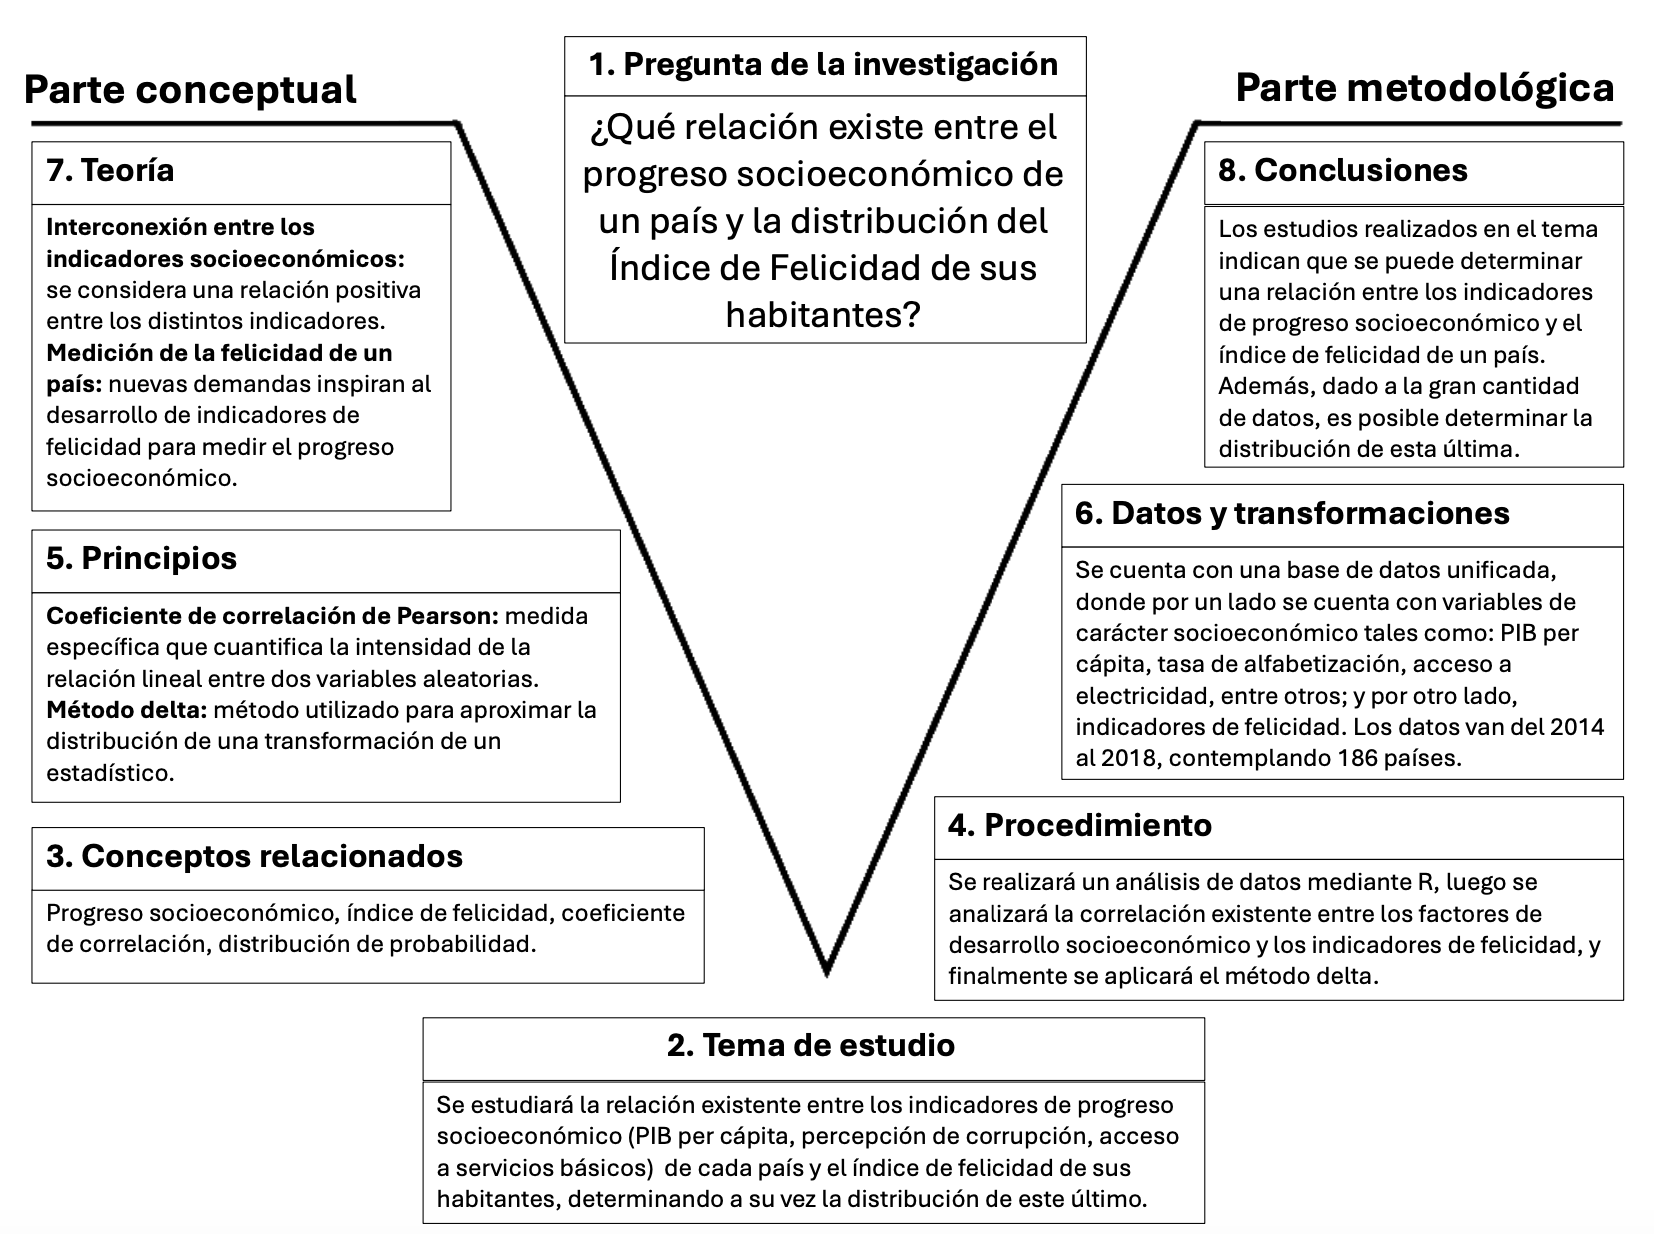
\includegraphics[width = 17cm]{figures/uve_de_gowin.png}
    \end{figure}

\pagebreak

\section{Parte de escritura}
\textbf{¿Qué relación existe entre la distribución del índice de felicidad y el progreso socio económico de un país?} \\

La relación que existe entre el índice de felicidad y el progreso socio económico medida con respecto a distintas variables representa un alto grado de utilidad para la comprensión de como afectan distintas variables a la felicidad que se experimenta en el país. Esto se presenta de interés para la toma de decisiones gubernamentales e implementación de políticas publicas, con el fin de mejorar la vida de los habitantes de un territorio y maximizar el bienestar social en este.\\
    
Los estudios actuales denotan la existencia de una relación entre la felicidad y el progreso económico, algunos de estos casos presentan un crecimiento de la felicidad de la cual se goza a medida que aumenta el ingreso, como lo es el caso de Perú de la forma en la que expresa Tinoco, (2020) "Un punto interesante sobre el estudio de esta relación es que no parece existir un punto de saciedad', es decir, un umbral o nivel límite donde un mayor ingreso personal no propicie mayor felicidad. Los datos y estudios realizados refieren que la capacidad del ingreso de influir sobre el bienestar no tiene límites." En el caso de Perú, se observa una relación positiva entre el ingreso y la felicidad, a tal punto de que no se observa una cota superior en la capacidad del ingreso en su influencia hacia la felicidad.\\
    
Mientras que el caso contrario también se encuentra presente, el cual se resume en una disminución de la felicidad a pesar de un aumento de variables económicas, en el caso de Butan, explicado por Aguilar, (2010) "De hecho, la correlación, en este caso negativa, es bastante elevada; del -71 \% en términos absolutos. Ha habido un crecimiento económico, no obstante no ha aumentado la satisfacción a nivel general." Un aumento de factores económicos presentó un efecto contradictorio en Butan durante el periodo del 2006-2009 con respecto al fenómeno observado en Urug\"uay.\\

Estos dos comportamientos se encuentran presentes a lo largo de los territorios que conforman las naciones, por lo cual se ha establecido como tarea principal, realizar un análisis de los datos recopilados de los distintos países, así como estudiar la correlación que existe entre las distintas variables presentes que funcionan como métricas del progreso económico y la felicidad. Como expresa de la siguiente forma Tinoco, (2020) "El estudio de la relación entre la felicidad y variables económicas como el ingreso, el desempleo y la inflación; este tipo de investigación ha generado una abundante XV." Relacionar la felicidad con distintas variables económicas es un proceso que se ha llevado a cabo de forma abundante en distintos países.
bibliografía durante los pasados 20 años.\\

\pagebreak
    
Además de realizar el análisis de datos y correlación entre las distintas variables, se busca desarrollar intervalos de confianza, así como encontrar la distribución que siguen las distintas variables económicas con respecto a la felicidad. De la forma en la cual lo expresa Candia, (2005) 

\begin{displayquote}
    El intervalo de confianza describe la variabilidad entre la medida obtenida en un estudio y la medida real de la población (el valor real). Corresponde a un rango de valores, cuya distribución es normal y en el cual se encuentra, con alta probabilidad, el valor real de una determinada variable. Esta «alta probabilidad» se ha establecido por consenso en 95\%.
\end{displayquote}

    

Esto con el fin de establecer un intervalo de confianza con respecto a los índices de correlación obtenidos para las distintas variables. Esto con la intención de obtener una mayor comprensión acerca de la correlación existente, dando lugar a resultados con una base más solida.\\


Finalmente se va a encontrar la distribución que presenta la variable de la felicidad ya que tanto la composición de esta como su relación con distintas variables económicas presenta una naturaleza compleja. Se desea hallar la distribución con el fin de presentar información mas completa y estructurada. Además de que se presenta una mayor facilidad a la hora de identificar patrones y la forma en la que se relacionan distintas variables.\\


El estudio de análisis de datos y correlación que se desea llevar a cabo se presenta como un problema complejo debido a las distintas formas que pueden influir las variables en la felicidad de un territorio en especifico, por lo cual es de suma importancia el llevar a cabo un trabajo ordenado y estructurado, que tome en cuenta intervalos de confianza que permitan estimar la variabilidad presente, y la naturaleza de las distribución de la felicidad para tener una visión más completa.

%
% --- Acá termina el texto ---
%

\label{EndOfText}

\newpage
\pagenumbering{Roman}
\fancyfoot[C]{Page \thepage\ of \pageref{endOfDoc}}
\thispagestyle{fancy}

\addcontentsline{toc}{section}{Índice de figuras}
\listoffigures
\thispagestyle{fancy}

\addcontentsline{toc}{section}{Índice de cuadros}
\listoftables
\thispagestyle{fancy}

\addcontentsline{toc}{section}{Referencias}
\nocite{*}
\bibliographystyle{apalike}
\bibliography{refs} 
\thispagestyle{fancy}

%\section{Apéndices}

\label{endOfDoc}
\end{document}